\documentclass[12pt,a4paper]{article}
\usepackage[T1]{fontenc}
\usepackage[utf8]{inputenc}
\usepackage{lmodern}
\usepackage{microtype}
\usepackage{mathtools}
\usepackage{amssymb,amsmath}
% Aumenta lo spacing tra equazioni su più righe
% nell'ambiente equation, rendendolo scalabile in base alla dimensione del testo
\setlength{\jot}{3ex}
\usepackage[makeroom]{cancel}
\usepackage{siunitx}
\usepackage{relsize}
\usepackage{tikz}
\usetikzlibrary{automata,positioning,calc,shapes,arrows}
\usepackage{multirow}
\usepackage{caption}
\captionsetup[figure]{font=small,labelfont=small}
\usepackage[english]{babel} 
\usepackage{float}
\usepackage[left=2.5cm,right=2.5cm,bottom=2cm,top=2cm,includeheadfoot]{geometry}
% Da scommentare per abilitare un ambiente Large
% migliore rispetto al Large normale
%\usepackage{environ}
%\NewEnviron{BiggerEquation*}{%
%\begin{equation*}
%\scalebox{1.5}{$\BODY$}
%\end{equation*}
%}
\linespread{1.2}

\DeclareMathOperator*{\argmax}{arg\,max}
\DeclareMathOperator*{\argmin}{arg\,min}
\newcommand*{\transp}{\mathsf{p}}

\title{Automata \& Queueing Systems}
\author{Francesco Casciola}

\usepackage{hyperref} %Per rendere l'indice cliccabile. Da rimuovere quando stampo.
\hypersetup{
	pdfprintscaling=None,
	colorlinks,
	citecolor=black,
	filecolor=black,
	linkcolor=blue,
	urlcolor=blue
}

\begin{document}
\maketitle
\tableofcontents
\newpage
\section{Introduction and State Automata}

A system with time-driven dynamics is a kind of system in which, even though events might occur, after that the system doesn’t stay in the same state, but this variates as the time goes on.

\bigskip
\noindent
A system with event-driven dynamics is a kind of system whose state variates only with the occurrence of certain events and it is constant in the time between an event and the next one. This produces a piecewise constant function in the time.

\paragraph{Discrete Event System} Dynamical system with discrete states and event-driven dynamics.

\paragraph{State Automaton} It’s a model through which Discrete Event Systems can be represented and it’s identified as a 5-tuple $(\mathcal{E},\mathcal{X},\Gamma,f,x_0)$ where:
\begin{itemize}
\item $\mathcal{E}$ is a discrete set of events.
\item $\mathcal{X}$ is a discrete set of states.
\item $\Gamma$ is a function taking values $\mathcal{X}\rightarrow 2^\mathcal{E}$, where $2^\mathcal{E}$ is the `power set’ of the set $\mathcal{E}$ and it represents the set of all the possible subsets of $\mathcal{E}$:
$$
\text{e.g. : }\mathcal{E}={a,b} \Rightarrow 2^\mathcal{E}=\{\emptyset, \{a\}, \{b\}, \{a,b\}\} \text{\hspace{1 cm};\hspace{1 cm}} dim(2^\mathcal{E}) = 2^{dim(\mathcal{E})}
$$
$\Gamma(x)$ represents the set of events that are possible in the state $x$. 
\item $f$ is a function taking values in $\mathcal{X}\times\mathcal{E}\rightarrow\mathcal{X}$ and defines the state transitions, such that $x' = f(x,e)$ is the next state when event $e\in\Gamma(x)$ occurs in the current state $x\in\mathcal{X}$.
\item $x_0\in\mathcal{X}$ is the initial state.
\end{itemize}
\begin{figure}[H]
	\centering
	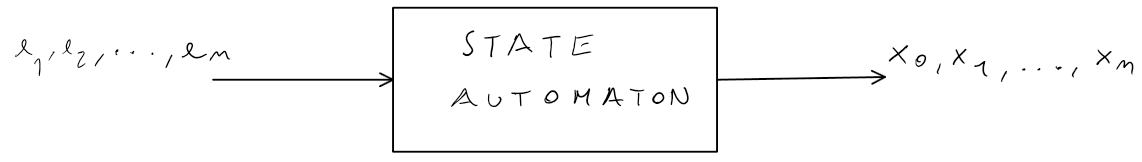
\includegraphics[width=\textwidth]{IMG/stateAut.png}
	\caption{State automaton block diagram.}
	\label{fig:stateAut}
\end{figure}
Don't confuse the model with the actual system because models introduce a certain degree of approximation with respect to the reality.

\paragraph{The concept of feasibility} When thinking about a real system there are many events that are possible and many others that aren’t. When modelling a system, the events that are extremely improbable (at a level that they can be considered impossible) must be excluded, but there are some events that are state-related that are actually impossible. For instance, a machine which is not working cannot complete a job. A sequence of events $(e_1,e_2,\dots,e_n)$ is \textbf{feasible} (could occur in reality) only if all the events of the sequence occur in states in which they are possible. In other words, the following conditions must hold:
\begin{align*}
e_k &\in \Gamma (x_{k-1}), \quad k = 1,2,\dots,n \\ 
x_k &= f(x_{k-1},e_k)
\end{align*}
Unfeasible sequences aren’t always obvious, which means that to find some of them it’s either necessary to have a deep knowledge of the system or to run a huge amount of model simulations (assuming that it’s realistic enough) to detect them.

\paragraph{State Automaton with outputs} It’s a model through which Discrete Event Systems can be represented and it’s identified as a 7-tuple $(\mathcal{E},\mathcal{X},\Gamma,f,x_0,\mathcal{Y},g)$ where:
\begin{itemize}
\item $(\mathcal{E},\mathcal{X},\Gamma,f,x_0)$ is a state automaton.
\item $\mathcal{Y}$ is a discrete set of outputs.
\item $g$ is a function taking values in $\mathcal{X}\rightarrow\mathcal{Y}$, such that $y=g(x)$ where $y\in\mathcal{Y}$ is the output corresponding to state $x\in\mathcal{X}$.
\end{itemize}

\section{Timed Automata}
\paragraph{Concept of time in DES} In a real system, when an event occurs, it’s also possible to know the time instant when this happens. When trying to introduce the concept of time in a State Automaton model, it’s important to remember:
\begin{itemize}
\item Time cannot be given as an input to the state automaton, since the inputs are independent of the system while time instants in which events occur depend on the system itself. 
\end{itemize}
This can be demonstrated by considering the execution of jobs on certain elements by a given machine as regulated by two different disciplines (while having the time as input): First-In-First-Out (FIFO) and Round-Robin (RR). The FIFO discipline is self-explanatory. The RR is based on the concept of `time slice’, which is the maximum time the machine dedicates to a certain element that needs processing before switching to the next one. In the case in which the time needed to complete the job on the first element is higher than the time slice, the partially processed element will be put back in the queue in last position.
Both the disciplines allow the machine to complete the job on all the elements, but, even if their times of arrival are the same, the times in which they are accepted in the system and the ones in which the processing on every single element terminates are different. This means that the time instants in which the events occur cannot be given as input to the system, as they depend on it.

\paragraph{Timed Automaton}
A solution to the problem presented in the past paragraph is to use as inputs, instead of the time instants, the duration of processes, at the end of which the events occur. This way, when the system enters a state $x$ in which a given event $e$ is possible, in the model it’s possible to start a process of a set duration. This process represents the \textit{event's lifetime} and when the lifetime depletes, the event occurs. Finally, the time instant when $e$ occurs is obtained as sum of the time instants in which the system enters the state x and the lifetime of the event e.
This allows us to define the \textbf{timed automaton} as a $6-$tuple $(\mathcal{E},\mathcal{X},\Gamma,f,x_0,V)$, where: 
\begin{itemize}
\item $(\mathcal{E},\mathcal{X},\Gamma,f,x_0)$ is a state automaton. 
\item $V$ is the \textit{clock structure} which is an array of `clock sequences’ of the various events:
$$
V=\{V_e : e\in\mathcal{E}\}, \quad V_e=\{v_{e,1}, v_{e,2}, v_{e,3},\dots\}
$$
\end{itemize}	
\noindent
Where $V_e$ is the clock sequence of event $e$ and $v_{e,i}$ is the lifetime of the $i$-th occurrence of event $e$. Please note that lifetimes must be $v_{e,i} \ge 0$ for the model to be representative of a real system.

\begin{figure}[H]
	\centering
	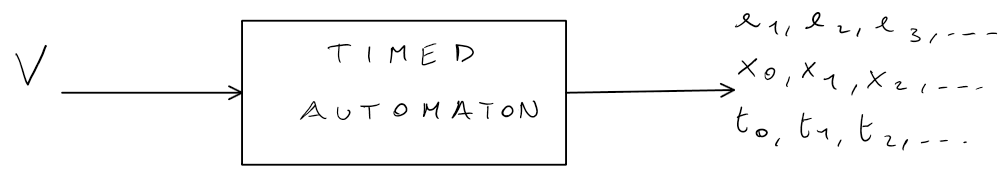
\includegraphics[width=\textwidth]{IMG/timedAut.png}
	\caption{Timed automaton block diagram.}
	\label{fig:timedAut}
\end{figure}

\paragraph{Residual Times} According to the definition of a Timed Automaton when entering a state in which an event is possible a process with a certain lifetime starts. Let’s consider the situation in which there are two lifetimes, related to two events $e_1$ and $e_2$, where $V_{e1}<V_{e2}$ that start when the system enters the state $x_{k-1}$. The event $e_1$ will occur first and the system will enter state $x_k$. If event $e_2$ is still possible in state $x_k$ then, instead of starting a new process with its lifetime, the `residual lifetime’ $y_{e2}=V_{e2}-V_{e1}$ is employed. If event $e_2$ is not possible there are two options: either dropping the current lifetime in order to start a new process when the event becomes possible again or keeping the residual lifetime in order to reuse it when the system enters a state in which $e_2$ is possible again. The choice between these options, in the model, depends on the behaviour of the system.

\paragraph{Notation for Timed Automata}
The `score’ of an event $e$ at the time $t$, denoted $n_e (t)$, is the number of lifetimes of the event e completed in the interval $[t_0,t]$. From now on the following notation will be used:
\begin{itemize}
\item With respect to event occurrences:
	\begin{itemize}
	\item $k$ is the event index $(k=1,2,3,\dots)$.
	\item $e_k$ is the $k$-th event.
	\item $x_k$ is the state reached after $e_k$ occurs.
	\item $t_k$ is the time when the $e_k$ occurs.
	\item $n_{e,k}$ is score of the event $e$ after the $k$-th event.
	\item $y_{e,k}$ is the residual lifetime of $e$ after the $k$-th event.
	\end{itemize} 
\item With respect to time:
	\begin{itemize}
	\item $t$ is the continuous time.
	\item $n_{e}(t)$ is score of the event $e$ after the time $t$.
	\item $x(t)$ is the state of the system at time $t$.
	\end{itemize} 
\end{itemize}
\paragraph{General algorithm for event timing} The algorithm works only when the following assumptions hold:
\begin{enumerate}
\item When an event $e$ doesn’t occur and it’s not possible in the next state, its residual lifetime is ignored and the next time event $e$ becomes possible a new total lifetime is taken from the corresponding clock sequence.
\item When event $e$ occurs, the next time it becomes possible a new total lifetime is taken from the corresponding clock sequence.
\item If the event $e$ doesn’t occur and it’s still possible in the next state, then its residual lifetime is used.
\end{enumerate}
\noindent
Under these assumptions, the algorithm is composed by the following steps:
\begin{enumerate}
\setcounter{enumi}{-1}
\item \textbf{Initialization:} for all the events $e\in\mathcal{E}$, if $e\in\Gamma(x_0)$ we consider $y_{e,0}=v_{e,1}$ and $n_{e,0}=1$. If $e\notin\Gamma(x_0)$, $y_{e,0}$ is undefined and $n_{e,0}=0$.
\item \textbf{Selection of the next event:} the next event is the one with the smallest residual lifetime.
$$
e_k = \argmin\limits_{\mathlarger{e\in\Gamma(x_{k-1})}} (y_{e,k-1}) = \text{arg} (y_{k-1}^*)
$$
\item \textbf{Determination of the time instant of the next event}
$$
t_k=t_{k-1}+y_{k-1}^*
$$
\item \textbf{State update}
$$
x_{k}=f(x_{k-1},e_{k})
$$
\item \textbf{Score update:}
for all the events $e\in\mathcal{E}$.
$$
n_{e,k}=
\begin{cases}
n_{e,k-1}+1 & \text{if a new total lifetime is used (ass. 1 and 2)} \\
n_{e,k-1} & \text{if the residual lifetime is used (ass. 3)}
\end{cases}
$$
\item \textbf{Update of the residual lifetimes:}
for all the events $e\in\mathcal{E}$.
$$
y_{e,k}=
\begin{cases}
v_{e,n_{e,k}} & \text{if } \left[\left(e\notin\Gamma(x_{k-1})\wedge e\in\Gamma(x_{k})\right)\vee\left(e=e_{k} \wedge e\in \Gamma(x_{k})\right)\right] \\
y_{e,k-1}-y_{k-1}^{*} & \text{if } \left[e\in\Gamma(x_{k-1})\wedge e\neq e_{k} \wedge e\in\Gamma(x_{k}) \right] \\
\end{cases}
$$
\item \textbf{Assign value $k+1$ to variable $k$ and go to step 1.}
\end{enumerate}

\section{Stochastic Timed Automata}
\paragraph{Concept of ubiquitous uncertainty}
In real systems there might be a degree of uncertainty which must be accounted for in the system's models. Suppose you have two machines which operate in parallel: how can you determine if they are both available, which one will start working when a piece arrives? Here’s a list of the elements in the Timed automaton which are subject to uncertainty:
\begin{itemize}
\item $f$: The example just described is a case of uncertainty in the state transition function.
\item $x_0$: Let’s consider a shop, if it opens at a given time $t_0$ and there are some people waiting for it to open, how long is the queue (state) at $t_0$? 
\item $V$: The processing times can vary depending on the request, it’s not always possible to know them in advance.
\end{itemize}
The need to introduce elements of uncertainty in the model bring to the definition of the next kind of state automaton.
\paragraph{Stochastic Timed Automaton}
It’s a model through which Discrete Event Systems with elements of uncertainty can be represented and it’s identified as a $6$-tuple $(\mathcal{E},\mathcal{X},\Gamma,P,p_0,F)$ where:
\begin{itemize}
\item $(\mathcal{E},\mathcal{X},\Gamma)$ are the same as for the timed automaton.
\item $\transp$ is a set of transition probabilities from a state to another. It substitutes $f$ and it’s defined as follows:
$$
\transp(x' \mid x,e) = P\left(X_{k+1} = x' \mid X_k = x, \, E_{k+1} = e\right), \qquad \forall e \in \Gamma(x) , \quad \forall x,x' \in \mathcal{X}
$$
This set of probabilities generalises the deterministic case, in fact if we have:
$$
\begin{matrix}
x'=f(x,e)&&\Rightarrow && P(x' \mid x,e)=1
\end{matrix}
$$
\item $\transp_0$ is a discrete random variable which defines the initial state probabilities:
$$
\transp_0(x)=P(x_0 = x), \quad \forall x\in \mathcal{X}
$$
\item $F$ is the stochastic clock structure and $F_e$ are the cumulative distribution functions of the lifetimes of event $e$:
$$
F = \{F_e : e \in \mathcal{E}\}, \quad F_e(t) = P(V_{e,i} \leq t)
$$
\end{itemize}
\noindent
We consider stochastic clock structure satisfying three assumptions:
\begin{itemize}
	\item The random variables $V_{e,i}$ are independent;
	\item The lifetimes $V_{e,i}$ of the same event are identically distributed;
	\item Lifetimes of \textit{different} events are independent.
\end{itemize}

\paragraph{Exponential Distribution}
When computing probabilities (like the probability of reaching a given state within a certain amount of time), since the lifetimes are random variables, it’s normally possible to know only the distributions of the total lifetimes, but not the one of the ones of the residual lifetimes. An exception is the one of exponential distribution which has some helpful properties that we are going to observe. The exponential distribution $X \sim \text{Exp}(1/\lambda)$ (where $1/\lambda$ is the location parameter and $\lambda$ is the rate) is defined as follows:
$$
\begin{matrix}
F_X(t)=P\left(X\leq t\right)=
\begin{cases}
1-e^{-\lambda t} & \textrm{if } t\geq 0 \\
0 & \textrm{otherwise} \\
\end{cases}
&&&
f_X(t)=\frac{dF_X(t)}{dt}=
\begin{cases}
\lambda e^{-\lambda t} & \textrm{if } t\geq 0 \\
0 & \textrm{otherwise} \\
\end{cases}
\end{matrix}
$$
Where $F_X(t)$ is the CDF and $f_X(t)$ is the pdf. The aforementioned properties are the following:
\begin{itemize}
\item \textbf{Memoryless property}: 
If the time between the occurrences $X$ of a given event is modelled through an exponential distribution and at the time $t$ the event hasn't occurred yet, the probability of the occurrence of the event (computed at a time $s>t$) does not depend $t$. In formulae:
$$
P(X>t+s \mid X>t)= P(X>s)
$$
\emph{Proof:}
\begin{equation*}
\begin{split}
P(X>t+s \mid X>t) &= \frac{P(X>t+s \textrm{ , } X>t)}{P(X>t)} = \frac{P(X>t+s)}{P(X>t)}= \\
= \frac{1-P(X\leq t+s)}{1-P(X\leq t)} &=\frac{1-F_X(t+s)}{1-F_X(t)} = \frac{e^{-\lambda (t+s)}}{e^{-\lambda t}} = e^{-\lambda s} = \\
&= 1 - P(X \leq s) = P(X>s)
\end{split}
\end{equation*}
\begin{flushright}
$\blacksquare$
\end{flushright}
\item \textbf{Extended memoryless property}:
The memoryless property can be defined in a more generic way by considering, instead of the time $t$, a generic time distribution $Y$, with support in $\left[0,\infty \right)$, independent from $X$:
$$
P(X>Y+s \mid X>Y)=P(X>s)
$$
\emph{Proof:}
\begin{equation*}
\begin{split}
P(X>Y+s \mid X>Y) = \frac{P(X>Y+s \textrm{ , } X>Y)}{P(X>Y)} = \frac{P(X>Y+s)}{P(X>Y)} 
\end{split}
\end{equation*}
Let's compute the numerator: $P(X>Y+s)$ is equal to the highlighted area $A$ in Figure \ref{fig:extmemlessarea} where the value of $X$ is greater than $Y+s$.
\begin{figure}[H]
\begin{center}
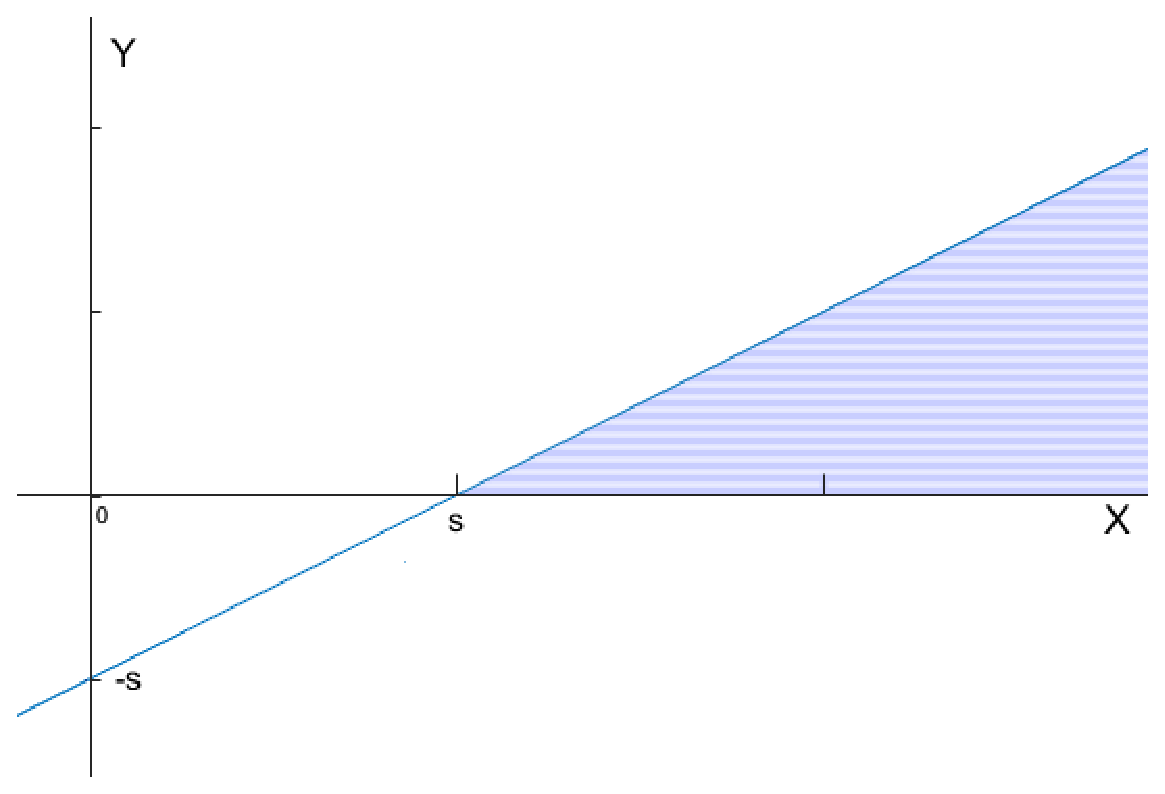
\includegraphics[width=0.5\textwidth]{IMG/CommArea.eps}
\caption{The highlighted area $A$ is the one for which $X-Y>s$}
\label{fig:extmemlessarea}
\end{center}
\end{figure}
This consideration allows us to proceed as follows:
\begin{equation*}
\begin{split}
P(X>Y+s) = P(X,Y\in A) = \int_{0}^{+\infty}dy\int_{y+s}^{+\infty}f_Y(y)\lambda e^{-\lambda x}dx= &\\
=\int_{0}^{+\infty}f_Y(y)dy\int_{y+s}^{+\infty}\lambda e^{-\lambda x}dx =\int_{0}^{+\infty}f_Y(y)
\left[-e^{-\lambda x}\right]^{+\infty}_{y+s}dy = &\\
=\int_{0}^{+\infty}f_Y(y)e^{-\lambda y}e^{-\lambda s}dy = e^{-\lambda s}
\int_{0}^{+\infty}f_Y(y)e^{-\lambda y}dy
\end{split}
\end{equation*}
Since the $s$ in the lower limit of integration in the innermost integral produces only a term 
$e^{-\lambda s}$ which can be put outside the integral, it's clear that
$$
\int_{0}^{+\infty}f_Y(y)e^{-\lambda y}dy = P(X>Y)
$$
Now it is easy to compute $P(X>Y+s \mid X>Y)$:
$$
\frac{P(X>Y+s)}{P(X>Y)} = \frac{e^{-\lambda s}\int_{0}^{+\infty}f_Y(y)e^{-\lambda y}dy }
{\int_{0}^{+\infty}f_Y(y)e^{-\lambda y}dy } = e^{-\lambda s} = 1-P(X\leq s) = P(X>s)
$$
\begin{flushright}
$\blacksquare$
\end{flushright}

\item \textbf{Superposition property}:
Let's consider the case in it's required to know, for independent events with exponentially distributed lifetimes $\left( X_i\sim Exp\left(\frac{1}{\lambda_i}\right)\right)$, the one that occurs first. The random variable that must be taken into account is:
$$
X=\min_{i=1,2,\dots,n}{\{X_i\}}
$$ 
The random variable $X$ is exponentially distributed with rate 
$$
\lambda '=\sum_{i=1}^{n}\lambda_i
$$
\emph{Proof:}
$$
P(X\leq t) = 1-P(X>t) = 1-P(\min_{i=1,\dots,n}{X_i}>t)
$$
From this last result, considering both the independence of the distributions and the fact that if the value $\min_i{\{X_i\}}$ is greater than $t$ then all the $X_i$ are, it's possible to proceed with the computation as follows:
$$
1-P(\min_{i=1,\dots,n}{X_i}>t) = 1-\prod_{i=1}^{n}{P(X_i>t)} = 1-\prod_{i=1}^{n}{1-P(X_i\leq t)} =
$$
$$
= 1-\prod_{i=1}^{n}{e^{-\lambda_{i}t}} = 1-e^{-\sum_{i}{\lambda_i t}} = 1-e^{-t\lambda'}
$$
Where $\lambda' = \sum_{i=1}^{n}{\lambda_i}$.
\begin{flushright}
$\blacksquare$
\end{flushright}
\end{itemize}
\newpage
\noindent
In addition to these properties, a `useful computation' (for the next topics) will be executed. Given two exponentially distributed random variables $X\sim Exp\left(\frac{1}{\lambda}\right),Y\sim Exp\left(\frac{1}{\mu}\right)$, let's compute the probability $P(X \leq Y+s)$:
\begin{figure}[H]
\begin{center}
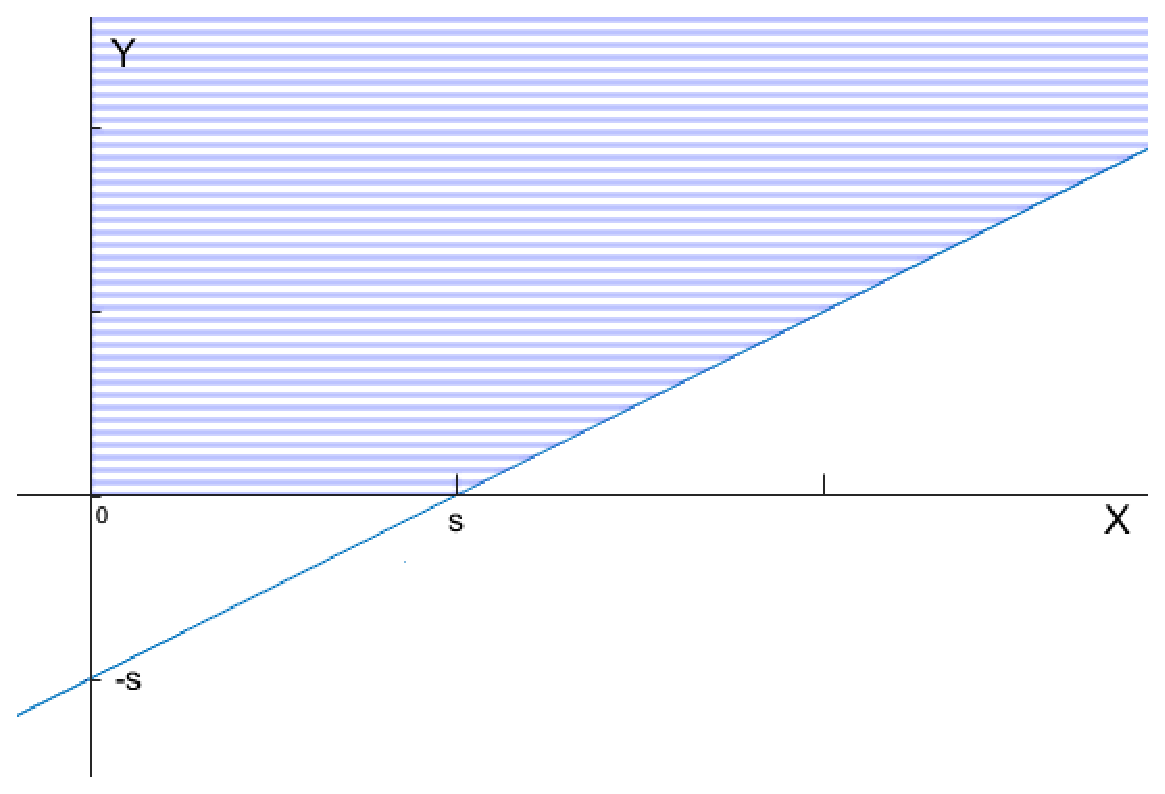
\includegraphics[width=0.5\textwidth]{IMG/CommArea2.eps}
\caption{The highlighted area is the one for which $X-Y\leq s$}
\label{Picture 2}
\end{center}
\end{figure}
$$
P(X \leq Y+s) = \int_{0}^{+\infty}dy\int_{0}^{y+s}\lambda e^{-\lambda x}\mu e^{-\mu y}dx
= \int_{0}^{+\infty}\mu e^{-\mu y}dy\int_{0}^{y+s}\lambda e^{-\lambda x}dx = 
$$
$$
=\int_{0}^{+\infty}\mu e^{-\mu y}\left[ -e^{-\lambda x}\right]_0^{y+s}dy
= \int_{0}^{+\infty}\mu e^{-\mu y}\left[ 1-e^{-\lambda(y+s)}\right]dy =
$$
$$
= \int_{0}^{+\infty}\mu e^{-\mu y}dy - e^{-\lambda s}\int_{0}^{+\infty}\mu e^{-\mu y} e^{-\lambda y}dy
= \left[-e^{-\mu y} + \frac{\mu e^{-\lambda s}}{\lambda + \mu}e^{-(\lambda+\mu)y}\right]_{0}^{+\infty} =
$$
$$
= 1-\frac{\mu e^{-\lambda s}}{\lambda + \mu} 
$$
Setting $s=0$ yields a closed-form formula for computing $P(X\leq Y)$ (skipping the entire chain of integration) which corresponds to the probability of lifetime X being less than lifetime Y.
\begin{equation}
\label{eq:xlessy}
P(X\leq Y)= \frac{\lambda}{\lambda + \mu}
\end{equation}
In the next chapter this last result will be used a lot, so it's important to keep it in mind.
\section{Stochastic Timed Automata With Poisson Clock Structure}
\paragraph{Poisson Counting Processes} It's a process which counts the occurrences of an event which is always possible. In particular, the `interarrival times' $T_i$ between any two occurrences of the same event are \textit{i.i.d.} and their distribution is:
$$
T_i\sim Exp\left(\frac{1}{\lambda}\right), \quad \lambda > 0
$$
\noindent
A Poisson counting process is defined as a discrete random variable $N_e(t,t+s)$ (it is a random variable because the interarrival times are, indeed, random variables) representing the number of occurrences of the event $e$ over the interval $\left( t,t+s\right]$. Given that the interarrival times are exponentially distributed, the probability mass function (pmf) of the Poisson counting process is:
\begin{equation*}
\begin{split}
P\left(N_e(t,t+s)=n\right)&, \qquad n = 0,1,2,\dots \\
P\left(N_e(t,t+s)=n\right)& = \frac{(\lambda s)^n}{n!}e^{-\lambda s}
\end{split}
\end{equation*}
Quite evidently, the pmf depends only on $s$ (due to the memoryless property), so:
\begin{equation}
\label{eq:poissonCountingDef}
P\left(N_e(s)=n\right) = \frac{(\lambda s)^n}{n!}e^{-\lambda s}
\end{equation}

\noindent
%From the PMF definition we can also reach the following result. Given $n$ \textit{i.i.d.} interarrival times $T_1,T_2,\dots,T_n \sim Exp\left(\frac{1}{\lambda}\right)$, $\lambda>0$:
%$$
%P\left(T_1,T_2,\dots,T_n \leq s\right) = 1-\sum_{m=0}^{n-1}P(N_e(s)=m)=1-\sum_{m=0}^{n-1}
%\frac{(\lambda s)^m}{m!}e^{-\lambda s}
%$$
%Given by the fact that, for the sum of the $n$ interarrival times to be less than $s$, the number of events occurred in the time $s$ has to be at least $n$.
Finally, it possible to compute the probability that at least $n$ occurrences of the event $e$ fall in the interval $s$:
$$
P\left(N_e(s) \geq n\right) = 1 - \sum_{m=0}^{n-1}P\left(N_e(s) = m \right) = 1 - \sum_{m=0}^{n-1} \frac{(\lambda s)^m}{m!}e^{-\lambda s}
$$
The first equality arises from the fact that the complement of $(n,n+1,n+2,\dots)$ is $(n-1,n-2,\dots)$. This is equivalent to splitting $s$ into $n$ intervals, each having width equal to $T_i$. Thus:
$$
P(T_1 + \dots + T_n \leq s) = 1 - \sum_{m=0}^{n-1} \frac{(\lambda s)^m}{m!}e^{-\lambda s}
$$

\paragraph{Stochastic Timed Automaton With Poisson Clock Structure}
It's a stochastic timed automaton 
$(\mathcal{E},\mathcal{X},\Gamma,\transp,\transp_0,F)$ where $F = \{F_e : e \in \mathcal{E}\}$, \textbf{with \textit{i.i.d.} events' lifetimes} and:
$$
F_e(t)=1-e^{-\lambda_e t}, \quad t\geq 0, \quad \lambda_e>0
$$
It's important to notice that there is no constraint about whether the events are always possible or not, this means that the `Poisson clock structure' doesn't refer to a Poisson counting process but to the fact that all the events have exponential interarrival times.
\emph{Moreover, for stochastic timed automata with Poisson clock structure, the residual lifetimes of the events follow the same distribution of the corresponding total lifetimes}. This last property can be proved through induction. The actual demonstration can be considered as homework by the reader.

\bigskip
\noindent
In stochastic timed automata with Poisson clock structure it's quite straightforward (compared to other models) to compute useful probabilities via closed-form formulas, such as:
\begin{enumerate}
\item $P(E_{k+1}=e \mid X_k=x)$ which is the probability that the next event $E_{k+1}$ (uppercase, since it's a random variable) will be $e$, given that the current state is $x$:
$$
P(E_{k+1}=e \mid X_k=x)=P\left(Y_{e,k} <
\min_{\left[
\begin{matrix}
e'\in \Gamma(x) \\
e'\neq e
\end{matrix}
\right]}
\left\lbrace Y_{e',k}\right\rbrace \right)
$$
Where the $Y$ random variables are the residual lifetimes of the feasible events in state $x$. Since the residual lifetimes follow exponential distribution, it's possible to use Equation \ref{eq:xlessy} and the superposition property to proceed with the computation:
\begin{equation}
\label{eq:inxnextstateise}
P\left(Y_{e,k} <
\min_{\left[
\begin{matrix}
e'\in \Gamma(x) \\
e'\neq e
\end{matrix}
\right]}
\left\lbrace Y_{e',k}\right\rbrace \right)
=\frac{\lambda_e}{\lambda_e+(\Lambda(x)-\lambda_e)}=\frac{\lambda_e}{\Lambda(x)}
\end{equation}
\noindent
Where $(\Lambda(x)-\lambda_e)$ is the rate of $Y_{e',k}$ since $\Lambda(x)$ is the sum of the rates of all the feasible events $e \neq e'$:
$$
\Lambda(x) = \mathlarger{\sum_{e \in \Gamma(x)}\lambda_e}
$$

\item $P(X_{k+1}=x' \mid X_k=x)$ which is the probability that the next state is $x'$, given that the current state is $x$:
$$
P(X_{k+1}=x' \mid X_k=x) \hspace{20pt}\underset{\textrm{rule}}{\overset{\textrm{total probability}}{=}}
$$
$$
=\sum_{e\in \Gamma(x)}{
\left[
P\left(
X_{k+1}=x' \mid X_k=x\textrm{, }E_{k+1}=e
\right)\cdot
P\left(
E_{k+1}=e \mid X_k=x
\right)
\right]
}=
$$
$$
=
\sum_{e\in \Gamma(x)}{
\left[
P\left(
X_{k+1}=x' \mid X_k=x\textrm{, }E_{k+1}=e
\right)\cdot
\frac{\lambda_e}{\Lambda(x)}
\right]}\triangleq
$$
$$
\underset{\textrm{for a more lean notation}}{\triangleq}
\sum_{e\in \Gamma(x)}{
\left[
\transp\left(x' \mid x,e
\right)\cdot
\frac{\lambda_e}{\Lambda(x)}
\right]}
$$
\end{enumerate}
These two results are quite good, but there are still more things that can be done. By defining 
$\mathcal{E}=\left\lbrace 1,2,\dots,m \right\rbrace$ and 
$\mathcal{X}=\left\lbrace 1,2,\dots,n \right\rbrace$
it's possible to define the following matrices and vector:
$$
P_E=
\left[
\begin{matrix}
P\left(E_{k+1}=1  \mid  X_k=1\right)&&
P\left(E_{k+1}=2  \mid  X_k=1\right)&&
\dots&&
P\left(E_{k+1}=m  \mid  X_k=1\right)\\\\
P\left(E_{k+1}=1  \mid  X_k=2\right)&&
P\left(E_{k+1}=2  \mid  X_k=2\right)&&
\dots&&
P\left(E_{k+1}=m  \mid  X_k=2\right)\\\\
\vdots&&
\vdots&&
\ddots&&
\vdots\\\\
P\left(E_{k+1}=1  \mid  X_k=n\right)&&
P\left(E_{k+1}=2  \mid  X_k=n\right)&&
\dots&&
P\left(E_{k+1}=m  \mid  X_k=n\right)
\end{matrix}
\right]
$$
\bigskip
$$
P_X=
\left[
\begin{matrix}
P\left(X_{k+1}=1  \mid  X_k=1\right)&&
P\left(X_{k+1}=2  \mid  X_k=1\right)&&
\dots&&
P\left(X_{k+1}=n  \mid  X_k=1\right)\\\\
P\left(X_{k+1}=1  \mid  X_k=2\right)&&
P\left(X_{k+1}=2  \mid  X_k=2\right)&&
\dots&&
P\left(X_{k+1}=n  \mid  X_k=2\right)\\\\
\vdots&&
\vdots&&
\ddots&&
\vdots\\\\
P\left(X_{k+1}=1  \mid  X_k=n\right)&&
P\left(X_{k+1}=2  \mid  X_k=n\right)&&
\dots&&
P\left(X_{k+1}=n  \mid  X_k=n\right)
\end{matrix}
\right]
$$
\bigskip
$$
\Pi_X(k)=
\left[
\begin{matrix}
P(X_k=1)&
P(X_k=2)&
\cdots&
P(X_k=n)&
\end{matrix}
\right]
$$
\bigskip
\noindent
So it's possible to redefine $P(X_{k+1} = x' \mid X_k = x)$ as the probability that the $k+1$-th state is $j$ as:
$$
P\left(X_{k+1}=j\right)=\sum_{\mathlarger{i\in \mathcal{X}}}
{
\underbrace{P\left(X_{k+1}=j  \mid  X_k=i\right)}_{(i,j)-\text{th}\text{ entry of }P_X}
\underbrace{P\left(X_k=1\right)}_{i-th\text{ entry of }\Pi_X(k)}
}
$$ 
$P(X_{k+1} = j)$ will be the $j$-th entry of the vector $\Pi_X(k+1)$ and of the product $\Pi_X(k) \cdot P_X$. 
So assuming that $\Pi_X(0)$ is known:
$$
\Pi_X(0)=
\left[
\begin{matrix}
\transp_0(1),&
\transp_0(2),&
\dots,&
\transp_0(n)
\end{matrix}
\right]
$$
$$
\begin{matrix}
\Pi_X(1)&=&\Pi_X(0) \cdot P_X\\
\Pi_X(2)&=&\Pi_X(1) \cdot P_X&=&\Pi_X(0) \cdot P_X^2\\
\Pi_X(3)&=&\Pi_X(2) \cdot P_X&=&\Pi_X(0) \cdot P_X^3\\
&&\vdots\\
\Pi_X(k+1)&=&\Pi_X(k) \cdot P_X&=&\Pi_X(0)P_X^k
\end{matrix}
$$
Likewise, it's possible to obtain the same result for the events: 
$$
P\left(E_{k+1}=j\right)=\sum_{\mathlarger{i\in\mathcal{X}}}{P\left(E_{k+1}=j \mid X_k=i\right)P\left(X_k=i\right)}
$$

$$
\Pi_E(k)=
\left[
\begin{matrix}
P\left(E_k=1\right),&
P\left(E_k=2\right),&
\dots,&
P\left(E_k=m\right)
\end{matrix}
\right]
$$

$$
\Pi_E(k+1)=\Pi_X(k)P_E=\Pi_X(0)P_X^kP_E
$$
With this result, it's finally possible to say that \emph{when using stochastic timed automata with Poisson clock structure, it's enough to know the matrices $P_X$ and $P_E$ and the vector $\Pi_X(0)$ to find all the future state and event probabilities}. 
\paragraph{Distribution of State Holding Times}
The state holding time $V(x)$ is a continuous random variable characterising the time spent by the system in state $x$. Notice that, while the system is in state $x$, there might occur events which do not trigger a state transition: this implies that $V(x)$ keeps increasing until the system leaves state $x$.
Let's compute the CDF of the state holding time, for a stochastic timed automaton with Poisson clock structure, and show that it is exponentially distributed with rate:
$$
\sum_{\mathlarger{e\in\Gamma(x)}}\lambda_e \left[
1-\transp\left(x \mid x,e\right) \right]
$$
\emph{Proof:}
The cdf of $V(x)$ is:
$$
P(V(x)\leq t) = 1-P(V(x)> t)
$$
Consider $P(V(x) > t)$ only:
\begin{equation*}
\begin{aligned}
&P(V(x)> t) = P\left(\textit{no state transitions over the }\left(0,t\right] \textit{ interval} \mid X(0)=x\right)= \\
&=P\left(\underset{e\in\Gamma(x)}\bigcap\textit{no state transition triggered by event e over }\left( 0,t\right] \mid X(0)=x\right)=\footnotemark \\
&=\prod_{e\in\Gamma(x)}
P\left(\textit{no state transition triggered by event e over }\left( 0,t\right] \mid X(0)=x\right)=\footnotemark \\
&=\prod_{e\in\Gamma(x)}
P\left(
\begin{aligned}
&\underset{n=0}{\overset{+\infty}\bigcup}
\textit{event e occurs exactly n times over } \left(0,t\right] \\
&\textit{and never triggers a state transition} \mid X(0)=x
\end{aligned}
\right) =\footnotemark \\
&=\prod_{e\in\Gamma(x)}\sum_{n=0}^{+\infty} P\left(
\begin{aligned}
&\textit{event e occurs exactly n times over } \left( 0,t\right]\\
&\textit{and never triggers a state transition} \mid X(0)=x
\end{aligned}
\right)=
\end{aligned}
\addtocounter{footnote}{-3} %1=n
\stepcounter{footnote}\footnotetext{Thanks to the independence of the events' lifetimes in Poisson clock structure}
\stepcounter{footnote}\footnotetext{It may occur more than once}
\stepcounter{footnote}\footnotetext{Union of disjoint events, you may sum them up}
\end{equation*}
\noindent
In this last probability the occurrences of an \textit{i.i.d} set of exponentially distributed random variables are counted, which is equivalent to a Poisson counting process. Therefore, it's possible to substitute Equation \ref{eq:poissonCountingDef} and multiply it by the probability that the system remains in $x$, given event $e$, exactly $n$ times:
\begin{equation*}
\begin{split}
&=\prod_{e\in\Gamma(x)}\sum_{n=0}^{+\infty}
\frac{\left(\lambda_e t\right)^{n}}{n!} \cdot e^{-\lambda_e t} \cdot \transp\left( x \mid x,e\right)^{n} = \\
&=\prod_{e\in\Gamma(x)}e^{-\lambda_e t}\sum_{n=0}^{+\infty} \frac{\left[(\lambda_e t)\cdot \transp (x \mid x,e)\right]^n}{n!}
=
\end{split}
\end{equation*}
\noindent
Now the last sum can be rewritten as $e^x=\sum_{n=0}^{+\infty}x^n/n!$ (Maclaurin series expansion):
\begin{equation*}
\begin{split}
&=\prod_{e\in\Gamma(x)}\exp(-\lambda_e t) \cdot
\exp(\lambda_e t \cdot \transp\left(x \mid x,e\right))= \\
&=\prod_{e\in\Gamma(x)}\exp(-\lambda_e \left[1 - \transp(x \mid x,e)\right] t)= \\
&= \exp\left(- \sum_{e\in\Gamma(x)} \lambda_e \left[1 - \transp(x \mid x,e)\right] t\right)
\end{split}
\end{equation*}
\noindent
Switching to the cdf of interest is straightforward (namely, the complement of $P(V(x)) > t$), thus:
\begin{equation*}
P\left(V(x)\leq t\right)=1- \exp\left(- \sum_{e\in\Gamma(x)} \lambda_e \left[1 - \transp(x \mid x,e)\right] t\right)
\end{equation*}
\begin{flushright}
$\blacksquare$
\end{flushright}
\newpage
\section{Markov Chains}
\paragraph{Stochastic Processes}
An example of a stochastic process was already proposed when talking about `Poisson counting process', now a slightly more formal definition will be given: \emph{`a stochastic process is a collection $\left\lbrace X\left(t\right) \right\rbrace_{t\in T} $
of random variables indexed by a time index $t\in T$'}, where $T$ is a time interval which can be either discrete or continuous.
The stochastic processes are actually classified depending on the nature of $T$:
\begin{itemize}
\item \textbf{if $T$ is discrete} (either finite or not) the process is a \emph{`discrete time stochastic process'} 
and it's also called \emph{`chain'}.
\item \textbf{if $T$ is continuous} the process is a \emph{`continuous time stochastic process'}.
\end{itemize}
To characterise stochastic processes it's necessary to provide joint distributions of all the possible $n$-tuples of the random variables which compose the process. Since this is really hard to realise, in these notes the stochastic processes will be used
only when the independence between the random variables holds, therefore with stochastic timed automata with Poisson clock structure. Finally, the independence concept in stochastic processes is defined as follows:

\bigskip
\noindent 
Given $X(t_1), X(t_2),\dots, X(t_n)$ random variables with $t_1<t_2<\dots<t_n \in T$ and $n=1,2,\dots$ the process is said \textit{`independent'} if all the $n-$tuples are independent. 

\bigskip
\noindent 
Let $x(t)$ be the realisation of the random variable $X(t)$, if the equality:
$$
P\left(X\left(t+s\right)=\overset{\sim}{x} \mid X\left(\tau\right)=
x\left(\tau\right),\hspace{5pt}\forall\tau\leq t\right)=
P\left(X\left(t+s\right)=\overset{\sim}{x} \right)
$$
holds, the process is independent. This means that the history of the past evolution of the system is irrelevant for predicting the future evolution ($t+s$ is called \textit{prediction horizon}).
\paragraph{Continuous Time Homogeneous Markov Chains (CTHMC)} are a subset of a kind of stochastic processes called `Markov processes' for which the definition of process independence is more relaxed than the standard one just given. If the condition:
$$
P\left(X(t+s)=\overset{\sim}{x} \mid X(\tau)=
x(\tau),\;\forall\tau\leq t\right)=
P\left(X(t+s)=\overset{\sim}{x} \mid X(t)=x(t)\right)
$$
holds, the process is independent. This definition allows the stochastic processes whose next realisation depends only on the current one to be called independent (\textit{`Markov property'}).

\bigskip
\noindent
The Continuous Time Homogeneous Markov Chains is a stochastic process with the following properties:
\begin{itemize}
\item $T=\mathbb{R}^+\Rightarrow\left\lbrace t\in\mathbb{R}:\;t\geq 0\right\rbrace $ (\textbf{Continuous Time}).
\item $X(t)\in \mathcal{X}=\left\lbrace 1,2,\dots\right\rbrace$ (\textbf{Chain}).
\item \textbf{Markov property} since it is a chain.
\item \textbf{Homogeneity}: the transition function depends only on the prediction horizon
$$
P\left(X(t+s)=j \mid X(t)=i\right) = P\left(X(t'+s)=j \mid X(t')=i\right),\;\forall t\neq t'
$$
Thus it can be rewritten as:
$$
\transp_{i,j}(s) = P\left(X(t+s)=j \mid X(t)=i\right)
$$
\end{itemize} 
\paragraph{Chapman-Kolmogorov Equation}
Please notice that $x(t)\in \mathcal{X}$ implies that the process' random variables realisations are the states of the system modelled as a CTHMC. So, let's try to compute the probability that, given a current state $i$, after a time $s$ the state will be $j$:
$$
\transp_{i,j}(s) = P\left(X(t+s)=j \mid X(t)=i\right)
$$
\begin{figure}
\begin{center}
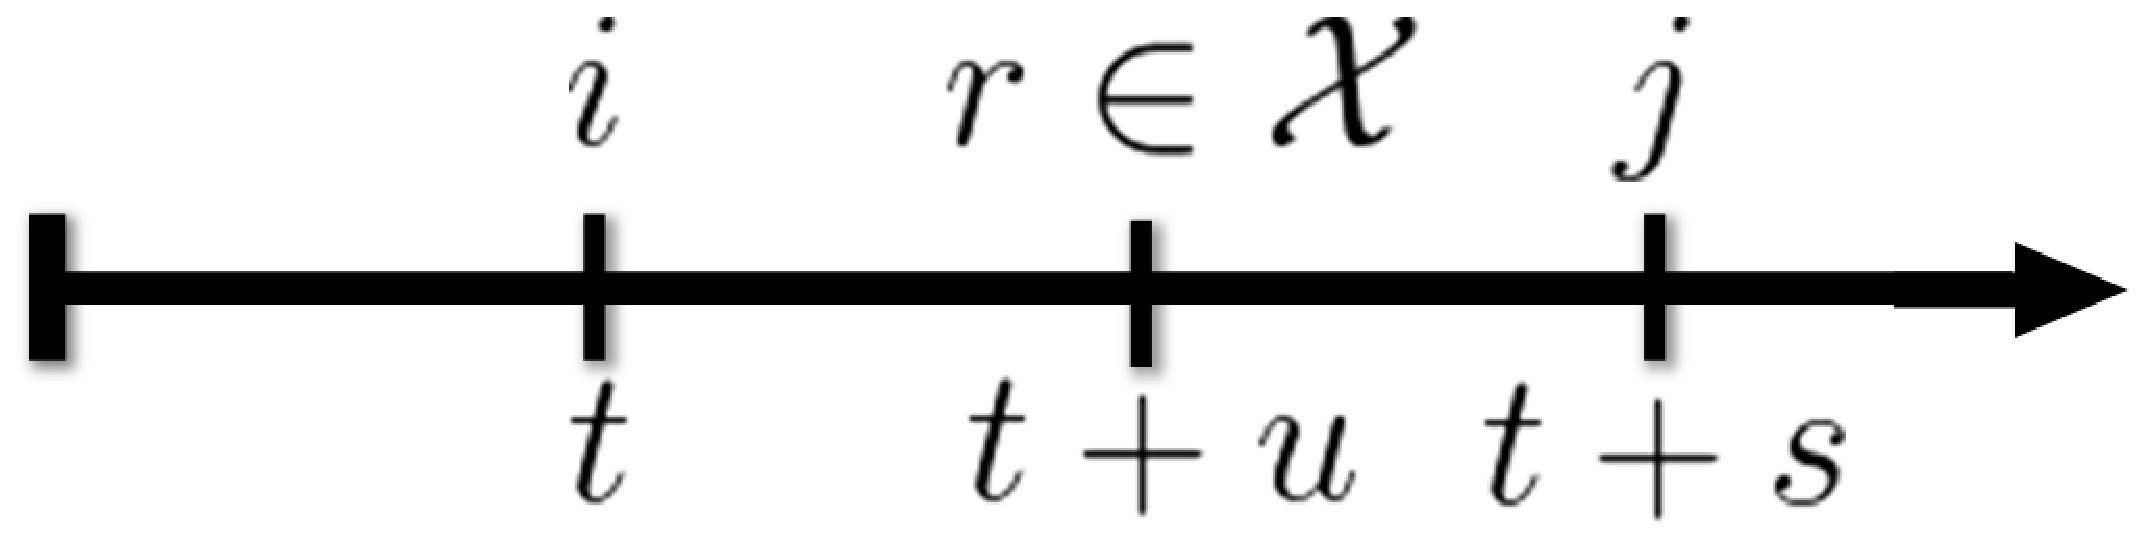
\includegraphics[width=0.35\textwidth]{IMG/CTHMC1.eps}
\caption{At time $t$ the current state is $i$. At $t+s$ the next state is $j$, while at $t+u$ the state is $r \in \mathcal{X}$ which can be $i$, $j$ or any other state.}
\label{fig:chapmanTimeDiagram}
\end{center}
\end{figure}
\noindent
In order to execute the computation, let's consider the case in Figure \ref{fig:chapmanTimeDiagram}:
\begin{equation*}
\begin{aligned}
\transp_{i,j}(s)&=P\left(X(t+s)=j \mid  X(t)=i\right)=\footnotemark \\
&=\sum_{r\in\mathcal{X}}P\left(X(t+s) = j \mid X(t+u) = r, \, X(t) = i\right) \cdot P\left(X(t+u) = r \mid X(t) = i\right) = \footnotemark \\
&=\sum_{r\in\mathcal{X}}P\left(X(t+s) = j \mid X(t+u) = r\right) \cdot P\left(X(t+u) = r \mid X(t) = i\right) = \\
&=\sum_{r\in\mathcal{X}}\transp_{r,j}(s-u)\cdot\transp_{i,r}(u)
\end{aligned}
\footnotetext{By applying the total proability rule}
\footnotetext{By applying the Markov property}
\end{equation*}
\noindent
The equality:
\begin{equation}
\label{eq:chapmanKDef}
\transp_{i,j}(s) = \sum_{r\in \mathcal{X}}\transp_{i,r}(u)\cdot \transp_{r,j}(s-u)
\end{equation}
is known as `Chapman-Kolmogorov equation'. As seen for the stochastic timed automata with Poisson clock structure, also here it's possible to define a matrix for the transition probabilities $\transp_{i,j}(s)$. Let's call this matrix $H(s)$:
$$
H(s)=\left[
\begin{matrix}
\transp_{1,1}(s)&\transp_{1,2}(s)&\cdots \\
\transp_{2,1}(s)&\transp_{2,2}(s)&\cdots \\
\vdots&\vdots&\ddots
\end{matrix}
\right]
$$
This matrix has some important properties:
\begin{enumerate}
\item The sum of the elements along any row of $H(s)$ is 1.
\item As a result of the previous property, if $s=0$ then the probability that the state does not change is 1, therefore $\transp_{i,i} = 1$ and $\transp_{i,j} = 0, \; j \neq i$:
$$
H(0)=I
$$
\item Since $\transp_{i,j}(s)$ is the generic element of matrix $H(s)$, from Equation \ref{eq:chapmanKDef} one notices that $H(s)$ equals the matrices product $H(u)$ by $H(s-u)$ (matrix form of the Chapman-Kolmogorov equation):
$$
H(s)=H(u) \cdot H(s-u)
$$
\end{enumerate}
From the last property it's possible to define the derivative of $H(s)$:
$$
\frac{dH(s)}{ds}=H(s) \cdot Q, \quad Q\triangleq\lim_{ds\rightarrow 0}\frac{H(ds)-I}{ds}
$$
\emph{Proof}:
We would like to obtain the difference quotient. Let's consider an infinitesimal difference $ds$:
\begin{equation*}
\begin{aligned}
&H(s+ds)=H(s)H(ds)= \footnotemark \\ &\frac{H(s+ds)-H(s)}{ds}=\frac{H(s)H(ds)-H(s)}{ds}
\end{aligned}
\footnotetext{By subtracting H(s) from both sides and dividing by ds}
\end{equation*}
Taking the limit for $ds\rightarrow 0$ yields the difference quotient on the left-hand side:
\begin{equation*}
\begin{aligned}
\lim_{ds\rightarrow 0}\frac{H(s+ds)-H(s)}{ds} = \lim_{ds\rightarrow 0}\frac{H(s)H(ds)-H(ds)}{ds}
\end{aligned}
\end{equation*}
Thus:
$$
\frac{dH(s)}{ds}=H(s) \cdot \lim_{ds\rightarrow 0}{\frac{H(ds)-I}{ds}}
$$
The right-hand side limit has an indeterminate form $0/0$ since $H(0)=I$, then
$$
(I-I)/ds \xrightarrow{ds\rightarrow 0} 0/0
$$
Let's \textit{assume that the limit exists} and let's call it $Q$. Since all the elements involved in the limit are matrices, also $Q$ will be a matrix (as a side note, matrix $Q$ can be estimated on the field by performing measurements on the system). Finally, taking into account property $\#2$ it's possible to define the following Cauchy problem:
$$
\begin{cases}
\dfrac{dH(s)}{ds}=H(s) \cdot Q\\ 
H(0)=I
\end{cases}
$$
Whose solution is:
$$
H(s)=e^{Qs}, \quad e^{Qs}=\sum_{n=0}^{+\infty}{\frac{(Q \cdot s)^n}{n!}}
$$ 
Where $e^{Qs}$ is the matrix exponential. Now we need to validate our initial assumption on the existence of $Q$. Starting from the initial definition of matrix $Q$, substitute the matrix exponential:
\begin{equation*}
\begin{aligned}
&\lim_{ds\rightarrow 0}\frac{H(ds)-I}{ds} = \lim_{ds\rightarrow 0}\frac{e^{Qds}-I}{ds}\overset{\text{Taylor}}{\underset{1^{st}\text{ order}}{=}} \\
&\lim_{ds\rightarrow 0}\frac{(I+Qds+o(ds))-I}{ds}=\lim_{ds\rightarrow 0}\frac{Q\cancel{ds}}{\cancel{ds}}+\cancelto{o(1)}{\frac{o(ds)}{ds}} = Q
\end{aligned}
\end{equation*}
Due to the last equality, it is clear that the result is consistent with the initial assumption.
\begin{flushright}
$\blacksquare$
\end{flushright}
\newpage
\subsection{The Q Matrix}
From the previous proof, it's hard to obtain any direct information about $Q$, so this section will be dedicated to the properties of the $Q$ matrix. To start with, this matrix is called `\emph{Transition Rate Matrix}':
$$
Q=\left[
\begin{matrix}
q_{1,1} & q_{1,2} &  \cdots \cr
q_{2,1} & q_{2,2} &  \cdots \cr
\vdots & \vdots &  \ddots
\end{matrix}
\right]
$$
where the generic element $q_{i,j}$ is called transition rate (their dimension is \si{\per\second}). Since the need of defining $Q$ came from the computation of the derivative of the matrix $H$, the properties of $H$ have been used to define the ones of $Q$. Let's start from the property of $H$ about the sum along any row being always $1$. Said $\textrm{\underline{\textbf{1}}}$ 
the vector $(1,1,1,\dots,1)^T$:
$$
H(s)\cdot \textrm{\underline{\textbf{1}}} = \textrm{\underline{\textbf{1}}}
\hspace{15pt}
\overset{\textrm{taking the derivative}}{\underset{\textrm{of both the sides}}{\Rightarrow}}
\hspace{15pt}
\underbrace{\frac{d\left(H(s)\right)}{ds}}_{H(s)Q}\textrm{\underline{\textbf{1}}}
\hspace{5pt}+\hspace{5pt}
\underbrace{\frac{d\textrm{\underline{\textbf{1}}}}{ds}}_{
=\hspace{2pt}O}H(s)
\hspace{5pt}=\hspace{5pt}
\underbrace{\frac{d\textrm{\underline{\textbf{1}}}}{ds}}_{=\hspace{2pt}O}
\hspace{5pt}\Rightarrow
$$
$$
\Rightarrow\hspace{5pt}
H(s)Q\cdot \textrm{\underline{\textbf{1}}}\hspace{5pt}=\hspace{5pt}O
\hspace{15pt}
\overset{s\rightarrow 0}{\underset{H(0)\hspace{2pt}=\hspace{2pt}I}{\Rightarrow}}
\hspace{15pt}
Q\cdot \textrm{\underline{\textbf{1}}}\hspace{5pt}=\hspace{5pt}O
$$

\bigskip
\noindent
Where $O$ is the vector $\left(0,0,0,\dots,0\right)$. From this final result it's clear that:

\bigskip\noindent
\underline{\emph{The sum along every row of $Q$ is always $0$.}} $\quad(\star )$

\bigskip\noindent
This property has an important implication: 
\emph{One of the eigenvalues of $Q$ it's always $0$}, since summing to one of the columns of $Q$ all the other columns will produce $O$. Therefore, the property $(\star )$ implies the linear dependency of one of the columns and, since the number of zero eigenvalues is equal to the dimension of the kernel \footnote[2]{$dim(ker(Q))=dim(Q)-rank(Q)$}, one of the eigenvalues will always be $0$.

\bigskip\noindent
So, keeping in mind the property $(\star )$, let's proceed with the definition of the generic coefficient $q_{i,j}$. At the moment, only the case in which $i\neq j$ will be considered. Let's start with the first order Taylor's representation of $H(ds)$, with $ds\rightarrow 0$:
$$
H(ds) \hspace{5pt} =\hspace{5pt}e^{Qds}
\hspace{5pt}
\overset{\textrm{Taylor}}{\underset{1^{st}\textrm{ order}}{=}}
\hspace{5pt}
I+Qds+o(ds)
$$ 

\bigskip\noindent
So, reducing this last equation to the coefficients of the matrices involved, the result will be 
(always under the condition $ds\rightarrow 0$):
$$
\transp_{i,j}(ds)=q_{i,j}ds+o(ds)
$$
Looking at the equation it's clear that \underline{\emph{all the $q_{i,j}$ with $i\neq j$ are non-negative}}, since $\transp_{i,j}(s)\geq 0$ (being a probability), $ds\geq 0$ (as it represents time, which cannot be negative) and $o(ds)$ goes to zero with $ds\rightarrow 0$. 
\newpage
\noindent
The non-negativity of $q_{i,j}$ and the property $(\star )$, impose that:

\bigskip\noindent
\underline{\emph{All the coefficients $q_{i,i}$ of the main diagonal of $Q$ must be non-positive}}, and in particular:
$$
q_{i,i}
\hspace{5pt}=\hspace{5pt}-
\sum_{j\neq i}{q_{i,j}}
$$

\paragraph{Physical Representation Of The Transition Rates}
On a physical level the elements of the $Q$ matrix have two different meanings, depending on whether they are on the main diagonal or not:
\begin{itemize}
\item The elements on the main diagonal define the rate of the distribution of the state holding times (which are exponentially distributed) of the system and, in particular:
$$
E\left[V(i)\right]=\frac{1}{-q_{i,i}}
$$
\item All the other elements are used, together with the ones from the main diagonal, to compute the overall state transition probability, independent from the time, from the generic state $i$ to the generic state $j\neq i$ with the formula:
$$
p_{i,j}=-\frac{q_{i,j}}{q_{i,i}}
$$
\end{itemize}
Let's start by computing the CDF of the state holding time of the generic state $i$, in order to provide a proof for the statement done about elements on the main diagonal:
$$
F_i(t)\hspace{5pt}\triangleq\hspace{5pt}
P\left( V(i)\leq t \right)
$$
And let's consider a small increment $dt$ of $t$ such that a state transition (only one) occurs in the time interval $(t,t+dt]$:
$$
F_i(t+dt)-F_i(t)\hspace{5pt}=\hspace{5pt}
P\left( t < V(i) \leq t+dt\right)\hspace{5pt}=\hspace{5pt}
P\left(V(i) \leq t+dt \mid  V(i)>t \right)\cdot 
\underbrace{P\left(V(i)>t\right)}_{1-F_i(t)}
$$
$$
\overset{\textrm{in particular}}{\Rightarrow}\hspace{10pt}
P\left(V(i) \leq t+dt \mid  V(i)>t \right)
\hspace{5pt}=\hspace{5pt}
\sum_{j\neq i}{\transp_{i,j}(dt)}
=
$$
$$
\overset{\textrm{Taylor}}{\underset{1^{st}\textrm{ order}}{=}}
\hspace{5pt}
\sum_{j\neq i}{q_{i,j}dt+o(dt)}
\hspace{10pt}
\Rightarrow
\hspace{10pt}
F_i(t+dt)-F_i(t)
\hspace{5pt}=\hspace{5pt}
\left[
\sum_{j\neq i}{q_{i,j}dt+o(dt)}
\right]
\left[
1-F_i(t)
\right]
$$ 
Dividing both the members of the last equation for $dt$ and computing the limit for $dt\rightarrow 0$
$$
\lim_{dt\rightarrow 0}{\frac{F_i(t+dt)-F_i(t)}{dt}}
\hspace{5pt}=\hspace{5pt}
\frac{d\left(F_i(t)\right)}{dt}
\hspace{5pt}=\hspace{5pt}
\lim_{dt\rightarrow 0}\frac{
\left[
\sum_{j\neq i}{q_{i,j}dt+o(dt)}
\right]
\left[
1-F_i(t)
\right]}{dt}
$$ 
$$
\frac{d\left(F_i(t)\right)}{dt}
\hspace{5pt}=\hspace{5pt}
\lim_{dt\rightarrow 0}{
\left[
\sum_{j\neq i}{\frac{q_{i,j}dt}{dt}+\frac{o(dt)}{dt}}
\right]
\left[
1-F_i(t)
\right]}
\hspace{5pt}=\hspace{5pt}
\sum_{j\neq i}{q_{i,j}}
\left[
1-F_i(t)
\right]
\hspace{5pt}=\hspace{5pt}
-q_{i,i}
\left[
1-F_i(t)
\right]
$$
\newpage
\noindent
In order to find $F_i(t)$, let's solve the following Cauchy Problem:
$$
\begin{cases}
\dfrac{d(F_i(t))}{dt}=-q_{i,i} \cdot [1-F_i(t)]\\
F_i(0)=0
\end{cases}
$$
Where $F_i(0)$ is the initial value of the generic state holding time $V(i)$. In order to compute the solution let's apply the following substitution:
$$
G_i(t)\hspace{5pt}\triangleq\hspace{5pt} 1-F_i(t)
\hspace{10pt}
\overset{\textrm{substituting }G_i(t) \textrm{ in}}
{\underset{\textrm{both the equations}}{\Rightarrow}}
\hspace{10pt}
\begin{cases}
\dfrac{d(G_i(t))}{dt}=-\dfrac{d(F_i(t))}{dt}=q_{i,i}\cdot G_i(t)\\
G_i(0)=1
\end{cases}
$$
The solution to this Cauchy problem is:
$$
G_i(t)=\exp(q_{i,i} \cdot t)
\Rightarrow
F_i(t)=1-G_i(t)=1-\exp(q_{i,i} \cdot t)
$$
This means that all the state holding times in CTHMC are exponentially distributed and, moreover that the rate of $F_i(t)$ is negative, namely $-q_{i,i}$. Computing the expected value of the distribution will return the result of the first statement.
\begin{flushright}
$\blacksquare$
\end{flushright}

\bigskip\noindent
Now the proof for the statement about the elements outside the main diagonal will be provided. Given two generic states $i$ and $j$, where $i\neq j$, and a generic time interval $(t, t+dt]$, let's compute the following probability:
\begin{equation}
\label{eq:qijtransition}
P(\textit{a transition from i to j occurs in the interval } (t, t+dt] \mid X_k=i)\hspace{5pt}=
\end{equation}
$$
=
\hspace{5pt}
P\left( V(i)>t\right)
P_{i,j}(dt)
\hspace{5pt}
=
\hspace{5pt}
\left[1-P\left( V(i)\leq t\right)\right]
\underbrace{P_{i,j}(dt)}_{
\overset{\textrm{Taylor }1^{\textrm{st}}\textrm{ order}}
{\overset{\Downarrow}{q_{i,j}dt+o(dt)}}}
\hspace{5pt}
\overset{dt\rightarrow 0}{=}
\hspace{5pt}
\left[1-\left(1-e^{q_{i,i} t}\right)\right]q_{i,j}dt
\hspace{5pt}
=
$$
\begin{large}
$$
\Rightarrow
\hspace{5pt}
P\left( V(i)>t\right)
P_{i,j}(dt)
\hspace{5pt}
=
\hspace{5pt}
e^{q_{i,i} t}q_{i,j}dt
$$
\end{large}

\noindent 
Let's now introduce another probability, which is the generic state transition probability from $i$ to $j$, without taking into account the time:
$$
p_{i,j}=P(X_{k+1}=j  \mid  X_k=i)
$$
$p_{i,j}$ can be obtained as sum of the probabilities like \ref{eq:qijtransition} computed for all the intervals of the kind 
$[t_n,t_n+dt_n]$, with $t_0=0$, $dt \rightarrow 0$, $n\in \mathbb{N}^+$:
$$
p_{i,j}
\hspace{5pt}
=
\hspace{5pt}
\int_0^{+\infty}{P\left( \textrm{a transition from }i\textrm{ to }j 
\textrm{ occurs in the interval} \left[ t, t+dt\right]
 \mid 
X_k=i
\right)} 
\hspace{5pt}
=
$$
$$
=
\hspace{5pt}
\int_0^{+\infty}{
e^{q_{i,i} t}q_{i,j}dt
}
\hspace{5pt}
=
\hspace{5pt}
q_{i,j}\left[ \frac{e^{q_{i,i}t}}{q_{i,i}}\right]_0^{+\infty}
\hspace{5pt}
=
\hspace{5pt}
-\frac{q_{i,j}}{q_{i,i}}
$$
\begin{flushright}
$\blacksquare$
\end{flushright}
\newpage
\subsection{Steady State Analysis}
Let's consider the `State Probability Vector' $\Pi(t)$, similar to the one in `\emph{Section $4$}':
$$
\Pi(t)\triangleq \left[
\begin{matrix}
&\Pi_1(t),& \Pi_2(t),& \Pi_3(t),& \dots&
\end{matrix}
\right]
$$ 
The `State Probability' of the generic $j-th$ state at time $t$ will be obtained as:

$$
\Pi_j\left(t\right)\hspace{5pt}=\hspace{5pt} P\left(x\left(t\right)=j\right)
\hspace{5pt}=\hspace{5pt} 
\sum_{i\in\mathcal{X}}{
\underbrace{
P\left( x \left( t \right) = j  \mid   x\left(0\right)=i\right)
}_{P_{i,j}(t)}
\cdot
\underbrace{
P\left(x\left(0\right)=i\right)
}_{\Pi_i(0)}
}\hspace{5pt}=\hspace{5pt}
\Pi(0)\cdot H_j(t)
$$

\noindent
Where $H_j(t)$ is the $j-th$ column of the matrix $H(t)$. This means that, given a time instant $t$, it's possible to compute all the state probabilities in one go by using:
$$
\Pi(t)\hspace{5pt}=\hspace{5pt}
\Pi(0)\cdot H(t)\hspace{5pt}=\hspace{5pt}
\Pi(0)\cdot e^{Qt}
$$
In the kind of system treated in this section the behaviour of the probabilities in time can be divided in two states: `Transient State' and `Steady State':
\begin{itemize}
\item \textbf{Transient State}: In order to analyse the behaviour of the system's state probabilities during the transient state, the derivative of $\Pi(t)$ must be computed:

$$
\frac{d\Pi(t)}{dt}
\hspace{5pt}=\hspace{5pt}
\Pi(0)\frac{dH(t)}{dt}
\hspace{5pt}=\hspace{5pt}
\Pi(0)H(t)Q
\hspace{5pt}=\hspace{5pt}
\Pi(t)Q
$$

\noindent
Which means that, to study the behaviour of the system in the transient state, it's enough to find the solution to the following Cauchy problem:

\begin{Large}
$$
\begin{matrix}
\begin{cases}
\frac{d\Pi(t)}{dt}=\Pi(t)Q\\
\Pi(0)=\Pi_0 \\
\end{cases}
\end{matrix}
$$
\end{Large}

\noindent
Where $\Pi_0$ is the initial state of the system.
\item \textbf{Steady State}: A system reaches steady state when every probability in the system starts varying less and instead converges asymptotically to a constant value. So in order to study steady state probabilities, it's necessary to focus on the following limit:

$$
\lim_{t\rightarrow \infty}{\Pi_i(t)}
$$
\end{itemize}
\newpage
\paragraph{Classification of States} in this paragraph some properties of the states, useful for the steady state analysis, will be explained:
\begin{itemize}
\item \textbf{Reachability}: A generic state $j$ is reachable from state $i$ if
$$
\exists\hspace{3pt}s : P_{i,j}(s)>0.
$$
Such concept can be also informally explained with the following definition: `\emph{it must exist a directed path from state $i$ to state $j$}'.
\item \textbf{Closure}: A subset $S\subseteq\mathcal{X}$ is `\emph{closed}' if 
$$
P_{i,j}=0,\hspace{10pt} \forall i\in S,\hspace{10pt} j\in\mathcal{X} \setminus S.
$$
Informally, it's possible to say that from the subset $S$ it's not possible to reach the states of the subset $\mathcal{X}\setminus S$:
\begin{figure}[H]
\begin{center}
$$
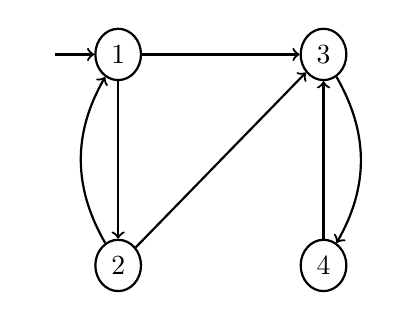
\begin{tikzpicture}
[
   thick,
   align=center,
   every state/.style={draw=black!60, fill=black!5}
]

\tikzset{state/.style = {shape=ellipse,draw, node distance=2cm}}
\tikzset{edge/.style = {->,> = angle 60, thick}}
% nodes
\node[state] (a) at  (0,0) {$1$};
\node[state,draw=none] (s) [left = 0.5cm of a] {};
\node[state] (b) [below =2cm of a] {$2$};
\node[state] (c) [right =2cm of a] {$3$};
\node[state] (d) [below =2cm of c] {$4$};
% arcs

\path[->]
   (s) edge  node[auto] {} (a)
   (a) edge node[auto] {} (b)
   (b) edge[bend left]  node[auto] {} (a)
   (a) edge node[auto] {} (c)
   (c) edge[bend left]  node[auto] {} (d)
   (d) edge node[auto] {} (c)
   (b) edge node[auto] {} (c)
   
;
\end{tikzpicture}
$$
\captionsetup{margin={60pt,60pt}}
\caption{\small the subset $\{3,4\}$ is an example of closed set, since once the system enters in state $3$ it's not possible that it will return to state $1$ or $2$ anymore.}
\end{center}
\end{figure}
\item \textbf{Irreducibility}: A closed subset $S\subseteq\mathcal{X}$ is called irreducible if every state of $S$ is reachable from other states of $S$.
\item \textbf{Recurrence}: Let's define the random variable $T_{i,i}$ as the time that takes to the system to return in state $i$. Let's also define the probability 
$\rho_i(t) \triangleq P\left( T_{i,i}<t\right)
$. Considering the limit for $t\rightarrow\infty$ of $\rho_i(t)$ it's possible to know if the system will ever return to state $i$.

$$
\rho_i\triangleq\lim_{t\rightarrow\infty}{\rho_i(t)}=
\begin{matrix}
\begin{cases}
1 & \textrm{ then the state will return (for }t\rightarrow\infty\textrm{) to the state i}\\
a<1 & \textrm{ then the state i is transient}\\
\end{cases}
\end{matrix}
$$

\noindent
Starting form the assumption that the state $i$ is recurrent, it's possible to realise a further classification. First of all it's important to remember that $\rho_i(t)$ is the CDF of $T_{i,i}$, so it's possible to define also the PDF $f_i(t)$ as $\rho_i(t)$'s derivative.
\newpage
So, now it's possible to compute the expected value $M_i$ of $T_{i,i}$, as follows:
$$
M_i\triangleq E\left[T_{i,i}\right]=\int_{0}^{+\infty}{t\cdot f_i(t)dt}=
\begin{matrix}
\begin{cases}
\infty & \textrm{then the integral doesn't converge and }\\
&\textrm{the state }i\textrm{ it's called `null recurrent'.}\\
a<\infty & \textrm{then the integral converges and }\\
& \textrm{the state }i\textrm{ it's called `positive recurrent'.}\\
\end{cases}
\end{matrix}
$$
In real applications the behaviours of null recurrent and transient states are the same, so the positive recurrent states are the only ones in which the system actually returns to the state $i$.
\end{itemize} 
From these definition it's possible to define two theorems and an important corollary:
\begin{enumerate}
\item If $i$ is a positive recurrent state and $j$ is reachable from $i$, then $j$ is positive recurrent.
\item If $S$ is a closed, irreducible and finite subset of $\mathcal{X}$, then all the states in $S$ are positive recurrent.
\item [2.1.] \underline{\emph{An irreducible and finite Markov Chain has only positive recurrent states.}}
\end{enumerate}
\paragraph{Steady State Analysis}
Let's now define the stationary probability vector:
$$
\Pi\triangleq \left[
\begin{matrix}
&\Pi_1,& \Pi_2,& \Pi_3,& \dots&
\end{matrix}
\right]
\hspace{10pt},\hspace{10pt}
\Pi_i\triangleq
\lim_{t\rightarrow\infty}{\Pi_i(t)}
$$ 
The actual definition of the stationary probability vector brings some problems that need to be solved before actually working with it, such as:
\begin{itemize}
\item Existence of the limit.
\item Conditions for the independence from the initial state $\Pi_0$.
\item Consistency of the probability vector, as the limit might exist but the probabilities might not sum up to $1$. 
\end{itemize}
A theorem (whose proof is not provided in these notes) states that for Continuous Time Homogeneous Markov Chains these problems, under precise conditions, can all be easily solved.

\bigskip
\noindent
\textbf{Theorem}: 

\noindent
For a CTHMC, which is irreducible and with all positive recurrent states, the limits
$$
\Pi_i=
\lim_{t\rightarrow\infty}{\Pi_i(t)}
$$
exist, with $\Pi_i>0,\hspace{4pt}\forall i\in\mathcal{X}$ and they are all independent of $\Pi_0$. Moreover, the vector $\Pi$ can be computed by solving the system of linear equations:

\begin{Large}
$$
\begin{matrix}
\begin{cases}
\Pi Q=0\\
\underset{i\in\mathcal{X}}{\sum{}}{\Pi_i=1}
\end{cases}
\end{matrix}
$$
\end{Large}
\newpage
\noindent
From this last theorem, keeping in mind also the corollary $\#2.1$ of the previous paragraph, the following corollary can be obtained:

\bigskip
\noindent
\textbf{Corollary}: 

\noindent
The previous theorem holds for irreducible and finite CTHMC.

\bigskip
\noindent
In both the theorem an the corollary the vector $\Pi$ can be found by solving the following system:
$$
\begin{matrix}
\begin{cases}
\Pi Q=0 & n \textrm{ equations}\\
\underset{i\in\mathcal{X}}{\sum{}}{\Pi_i=1} & 1 \textrm{ equation}
\end{cases}
\end{matrix}
$$
Where $n$ is the cardinality of $\Pi$. This means that there is a redundant equation, which can be found in $\Pi Q=0$, due to the fact that $Q$ doesn't have full rank since it has an eigenvalue $\lambda =0$. So, the constraint $\sum_{i\in\mathcal{X}}{\Pi_i=1}$ ensures both the consistency of the probability vector and the existence of a unique solution.
As a final clarification about the equations in the system, the set of equations given by $\Pi Q=0$ comes from the definition already treated for the transient state definition:
$$
\frac{d\Pi(t)}{dt}=\Pi(t)Q
$$ 
Since for $t\rightarrow\infty$ the state probabilities are expected to converge to constant values, their derivatives are expected to converge to zero, so:
$$
\frac{d\Pi(t)}{dt}=\Pi(t)Q \hspace{10pt} \overset{t\rightarrow\infty}{\Rightarrow}\hspace{10pt} \Pi Q=0
$$
\newpage
\paragraph{Equivalent CTHMC for Stochastic Timed Automata With Poisson Clock Structure}

\noindent A Stochastic Timed Automaton with Poisson Clock Structure $(\mathcal{E},\mathcal{X},\Gamma,P,p_0,F)$
is `stochastically equivalent' to a CTHMC $(\mathcal{X},Q,\Pi_0)$ which has:
\begin{itemize}
\item the same distributions for the state holding times:
$$
V_i \sim Exp\left(\frac{1}{-q_{i,i}}\right)
$$
\item the same state transition probabilities:
$$
p_{i,j}=\frac{q_{i,j}}{-q_{i,i}}
$$
\end{itemize}  
So, in order to find the equivalent Markov Chain for a Stochastic Timed Automaton with Poisson Clock Structure it's enough to:
\begin{itemize}
\item Compute the expected value of the state holding time for every state, and compute the $q_{i,i}$ as:
$$
q_{i,i}=-\frac{1}{E[V(i)]}=-\sum_{e\in\Gamma(i)}{\lambda_e\left[1-\transp(i \mid i,e)\right]}
$$
\item Compute the $p_{i,j}$ according to the frequentist probability in order to find the corresponding $q_{i,j}$ as:
$$
q_{i,j}=-q_{i,i}p_{i,j}=\sum_{e\in\Gamma(i)}{\lambda_e \transp(j \mid i,e)}
$$
\end{itemize}
Where $\lambda_e$ is the rate of the exponential distribution (since all the events lifetimes' distributions are exponential) of the event $e$.
\newpage
\section{Queueing Systems}
Queueing systems are a really important kind of discrete events systems and they can be treated using any of the models defined up to now. When looking for a representation for a queueing system, a really general one could be the following:

\begin{figure}[H]
\begin{center}
\begin{tikzpicture}
% draw the rectangular shape with vertical lines
\node[rectangle split, rectangle split parts=4,
draw, rectangle split horizontal,text height=1cm,text depth=0.5cm,inner ysep=0pt] (Q) {Queue};
% nodes
\node[circle,minimum size=1pt] (h0) [right =30pt of Q] {};
\node[draw,circle,minimum size=1.5cm] (s1) [label=above:{Server 1}] [above right =3cm of h0]{$S1$};
\node[draw,circle,minimum size=1.5cm] (s2) [label=above:{Server 2}] [below right =3cm of h0]{$S2$};
\node[circle,minimum size=1pt] (h1) [below right =3cm of s1] {};
% the arrows and labels
\draw[-] (Q.east) -- +(30pt,0) node[right] {};
\draw[->] (h0.west) -- +(2.20cm,2.75cm) node[left] {};
\draw[->] (h0.west) -- +(2.20cm,-2.75cm) node[left] {};
\draw[-] (s2.east) -- +(2.20cm,2.80cm) node[left] {};
\draw[-] (s1.east) -- +(2.20cm,-2.80cm) node[left] {};
\draw[->] (h1.east) -- +(30pt,0) node[left] {};
\end{tikzpicture}
\caption{\small Generic queueing system representation.}
\label{Picture 4}
\end{center}
\end{figure}
In order to define a queueing system, some parameters must be specified:
\begin{itemize}
\item \textbf{Structural Parameters}:
	\begin{itemize}
	\item Number of servers.
	\item Capacity of the queue.
	\end{itemize}
\item \textbf{Operating Policies}:
	\begin{itemize}
	\item Number of accepted customers and their `type' (so the kind of service they need).
	\item Scheduling Policy of the queue (FIFO, Round-Robin, Shortest Processing Time, ...).
	\item Conditions to accept new customers in the system.
	\end{itemize}
\item \textbf{Distributions of interarrival and sevice times}.
\end{itemize}
The choices made in the definition phase of a queueing system will affect its behaviour, especially the 
`\textit{effective production rate}'. When producing any kind of product (or providing any kind of service), this is done by expecting a certain demand for that product (or service). The queueing system must be designed in order to meet the demand, in particular the effective production rate $\mu_{eff}$ must be greater than the `\textit{demand rate}' $d$:
$$
\mu_{eff}\geq d
$$
\newpage
\paragraph{Kendall's Notation} can be used to describe queueing systems where there exists only one kind of customer. 
The notation is composed by the following set of parameters:
\begin{Large}
$$
A \hspace{3pt} / \hspace{3pt} B \hspace{3pt} / \hspace{3pt} m \hspace{3pt} / \hspace{3pt} K
/ \hspace{3pt} n \hspace{3pt} / \hspace{3pt} D
$$
\end{Large}

\noindent
Where:
\begin{itemize}
\item \textbf{A}: is the distribution of the interarrival times.
\item \textbf{B}: is the distribution of the service times.
\end{itemize}
The possible values for $A$ and $B$ are:
$$
\begin{matrix}
M & : & \textrm{Exponential distribution (\underline{Memoryless})} \cr
U & : & \textrm{Uniform distribution} \cr
G & : & \textrm{Generic distribution} \cr
D & : & \textrm{Deterministic distribution}
\end{matrix}
$$
\begin{itemize}
\item \textbf{m}: is the number of servers.
\item \textbf{K}: is the capacity of the system (therefore the capacity of the queue is $K-m$).
\item \textbf{n}: is the size of the population from which the customers come.
\item \textbf{D}: is the scheduling policy.
\end{itemize}
When one or more parameters are not specified it means that the model of the queueing system operates without taking into account the information deriving form them. In fact, in these notes, only systems that can be represented through the notation
$A/B/n/K$ are treated.

\paragraph{Queueing systems in steady state}
Before proceeding with the behaviour of queueing systems in steady state, it's necessary to provide some definitions. Let's consider the generic $k$-th customer entering a queueing system. The time spent by the customer in the system doesn't necessarily correspond to the time that took the system to process the customer request. So, said $Z_k$ and $W_k$ respectively the `service time' and the `waiting time' of the $k$-th customer in the system, the overall time spent in the system is called `system time' and it's defined as:
$$
S_k \triangleq W_k+Z_k
$$ 
Generally, the distribution of the system time it's different for every customer accepted in the system, but after a certain amount of customers accepted by the system, this might enter in a steady state. If a queueing system enters steady state, then the distributions of the system times will be the same for all the customers.
\newpage
\noindent
\textbf{Definition:}

\bigskip\noindent
If there exists a random variable $S$ such that:
$$
P\left( S\leq t\right)
\hspace{5pt}
=
\hspace{5pt}
\lim_{k\rightarrow \infty}
{P\left( S_k\leq t\right)}
\hspace{15pt}
,
\hspace{15pt}
\forall t
$$
Then the random variable $S$ describes the system time of a generic customer while the system is in steady state.

\bigskip\noindent
Using the same approach for $X(t)$, which is the number of customers in the system at time $t$:

\bigskip
\noindent
\textbf{Definition:}

\bigskip\noindent
If there exists a random variable $X$ such that:
\begin{equation*}
P(X = i) = \lim_{t\rightarrow \infty} P(X(t) = i), \quad \forall i
\end{equation*}
Then the random variable $X$ describes the number of customers in the system when this is in steady state. Moreover, always in steady state, since the number of customers in the system doesn't depend on the time anymore, then also its expected value $E\left[X(t)\right]$ doesn't:
$$
E\left[X(t)\right]
\hspace{5pt}
=
\hspace{5pt}
\sum_{i}
{
i \cdot P\left(X(t)=i\right)
}
\hspace{5pt}
\overset{t\rightarrow \infty}{=}
\hspace{5pt}
\sum_{i}
{
i \cdot P\left(X=i\right)
}
$$
From the rightmost result it comes out that $E\left[X(t)\right]=E\left[X\right]$.

\bigskip\noindent
In particular, from these definitions it's possible to define a necessary condition for the system to be in steady state. Said $\mu_{eff}$ the effective production rate and $\lambda_{eff}$ the effective arrival rate (rate of arrivals accepted in the system) at steady state the following condition must hold:
$$
\mu_{eff}\hspace{5pt}=\hspace{5pt}\lambda_{eff}
$$
This condition hold also for queueing networks, which are queueing systems composed by others queueing sub-systems. So, considering a system consisting of two stations in series, each of them composed by a machine preceded by a buffer, if the whole system reaches steady state the following conditions will hold:
$$
\mu_{eff,1}\hspace{5pt}=\hspace{5pt}\lambda_{eff,1}
\hspace{10pt}
,
\hspace{10pt}
\mu_{eff,2}\hspace{5pt}=\hspace{5pt}\lambda_{eff,2}
$$
When studying the steady state of a queueing system, an important parameter to take into account would be the `utilization' $U$, which is the fraction of time (over all the system activity time) in which the machine is actively working. If $U=1$ the machine it's always working, of course if $U=1$ for an observation time $t\rightarrow \infty$, then the machine is perfect. 

\bigskip\noindent
The utilization value is also used to obtain another parameter called \emph{throughput}, which is defined as the mean number of requests serviced during a time unit:
$$
throughput\hspace{5pt}=\hspace{5pt}U\cdot m\cdot \mu_{eff}
$$
In particular, on a single server system with $U=1$ the throughput is equal to $\mu_{eff}$.
\newpage

\paragraph{Little's Law}
Let's consider a queueing network at steady state and a curve $\Sigma$, closed around any fraction of the network (also the whole network can be considered an acceptable fraction). Let's consider only the portion of network within $\Sigma$ and let's define:
\begin{itemize}
\item $\lambda_{\Sigma}$ as the arrival rate for the arrivals which enter the curve $\Sigma$ (if $\Sigma$ surrounds the whole network $\lambda_{\Sigma}=\lambda_{eff}$).
\item $E[X_{\Sigma}]$ as the expected value of the number of customers within $\Sigma$ (if $\Sigma$ surrounds the whole network $E[X_{\Sigma}]=E[X]$).
\item $E[S_{\Sigma}]$ as the expected value of the time spent by a customer in $\Sigma$ (if $\Sigma$ surrounds the whole network $E[S_{\Sigma}]=E[S]$).
\end{itemize}
Little's Law states that:

\bigskip \noindent
\begin{Large}
$$
E[X_{\Sigma}]\hspace{5pt}=\hspace{5pt}\lambda_{\Sigma}\cdot E[S_{\Sigma}]
$$
\end{Large}

\bigskip \noindent
This law comes particularly handy since $E[S_{\Sigma}]$ it's often hard to compute directly, while instead it's easy to do it for the other two parameters.
\paragraph{PASTA Property}
It's another property for queueing systems. Let's define:
\begin{itemize}
\item $A(t)$ as the occurrence of an arrival in the system at the time $t$.
\item $\alpha_n(t)$ as the posterior probability that the state at time $t$ is $n$, knowing that at time $t$ an arrival occurs:
$$
\alpha_n(t)
\hspace{5pt}=\hspace{5pt}
P(X(t)=n \hspace{4pt} | \hspace{4pt} A(t))
$$
\item $\Pi_n(t)$ as the prior probability that the state at time $t$ is $n$:
$$
\Pi_n(t)
\hspace{5pt}=\hspace{5pt}
P(X(t)=n)
$$
\end{itemize}
Generally, $\alpha_n(t)\neq \Pi_n(t)$, but PASTA property states that:

\bigskip\noindent
\emph{If the arrivals are generated by a Poisson process and the lifetimes for arrivals and service terminations are independent then:}
$$
\alpha_n(t) \hspace{5pt}=\hspace{5pt} \Pi_n(t) \hspace{10pt},\hspace{10pt} \forall t,n
$$
Which means that it's possible to obtain, under these conditions, the posterior probability simply by computing the prior. Moreover, since the result of PASTA property holds $\forall t$, it can also be used when the system is in steady state.
\newpage

\paragraph{Ergodicity}
It's a property of stochastic processes $X_h(t)$ in which the ensemble average (average over $h$) and the time average are the same. In particular, when the system is in steady state, its stochastic behaviour won't depend on time anymore and therefore it can be considered ergodic. So, the only condition for ergodicity is that the system must be able to reach steady state.

\bigskip \noindent
The reason why ergodicity is such an interesting property is that it makes possible to compute, when the system is in steady state, the fraction of time spent in a certain state as the prior probability of being in that state and vice versa.



\end{document}